% This is LLNCS.DEM the demonstration file of
% the LaTeX macro package from Springer-Verlag
% for Lecture Notes in Computer Science,
% version 2.4 for LaTeX2e as of 16. April 2010
%
\documentclass{llncs}

% allows for temporary adjustment of side margins
\usepackage{chngpage}

% just makes the table prettier (see \toprule, \bottomrule, etc. commands below)
\usepackage{booktabs}

\usepackage[utf8]{inputenc}

% URL handling
\usepackage{url}
\urlstyle{same}

% footnotes
\usepackage{scrextend}

% Todos
%\usepackage[colorinlistoftodos]{todonotes}
%\newcommand{\ke}[1]{\todo[size=\small, color=orange!40]{\textbf{Kai:} #1}}
%\newcommand{\tb}[1]{\todo[size=\small, color=green!40]{\textbf{Thomas:} #1}}


%\usepackage{makeidx}  % allows for indexgeneration

%\usepackage{amsmath}
\usepackage{amsmath, amssymb}
\usepackage{mathabx}

% monospace within text
\newcommand{\ms}[1]{\texttt{#1}}

%\usepackage{listings}% http://ctan.org/pkg/listings
%\lstset{
  %numbers=left,numbersep=2mm,frame=single,mathescape,fontsize=\scriptsize
%}

% examples
\usepackage{fancyvrb}
\DefineVerbatimEnvironment{ex}{Verbatim}{numbers=left,numbersep=2mm,frame=single,fontsize=\scriptsize}

\newenvironment{gcotable-1}{
  \scriptsize
  \sffamily
  \vspace{0cm}
  \begin{tabular}{l|l|l|l|l|l}
  \hline
  \textbf{c. type} & \textbf{context concept} & \textbf{p. list} & \textbf{concepts} & \textbf{c. element} & \textbf{c. value} \\
  \hline

}{
  \hline
  \end{tabular}
}

\newenvironment{gcotable}{
  \scriptsize
  \sffamily
  \vspace{0cm}
	\begin{center}
  \begin{tabular}{l|l|l|l|l|l|l}
  \hline
  \textbf{c. type} & \textbf{context class} & \textbf{left p. list} & \textbf{right p. list} & \textbf{classes} & \textbf{c. element} & \textbf{c. value} \\
  \hline

}{
  \hline
  \end{tabular}
	\end{center}
}

\newenvironment{DL}{
  %\scriptsize
  %\sffamily
  \vspace{0cm}
	\begin{center}
  \begin{tabular}{r l}

}{
  \end{tabular}
	\end{center}
}

\newenvironment{evaluation}{
  %\scriptsize
  %\sffamily
  \vspace{0cm}
	\begin{center}
  \begin{tabular}{l|c|c|c|c|c|c}
  \hline
  \textbf{Constraint Class} & \textbf{DSP} & \textbf{OWL2-DL} & \textbf{OWL2-QL} & \textbf{ReSh} & \textbf{ShEx} & \textbf{SPIN} \\
  \hline

}{
  \hline
  \end{tabular}
	\end{center}
}

\newenvironment{evaluation-generic-overview}{
  %\scriptsize
  %\sffamily
  \vspace{0cm}
	\begin{center}
  \begin{tabular}{l|c|c}
  \hline
  \textbf{Constraint Classes} & \textbf{\#} & \textbf{\%} \\
  \hline

}{
  \hline
  \end{tabular}
  %\linebreak
	\end{center}
}

\usepackage{xspace}
% Einfache und doppelte Anfuehrungszeichen
\newcommand{\qs}{``} 
\newcommand{\qe}{''\xspace} 
\newcommand{\sqs}{`} 
\newcommand{\sqe}{'\xspace} 

% checkmark
\usepackage{tikz}
\def\checkmark{\tikz\fill[scale=0.4](0,.35) -- (.25,0) -- (1,.7) -- (.25,.15) -- cycle;} 

% Xs
\usepackage{pifont}

% Tabellenabstände kleiner
\setlength{\intextsep}{10pt} % Vertical space above & below [h] floats
\setlength{\textfloatsep}{10pt} % Vertical space below (above) [t] ([b]) floats
% \setlength{\abovecaptionskip}{0pt}
% \setlength{\belowcaptionskip}{0pt}

\usepackage{tabularx}
\newcommand{\hr}{\hline\noalign{\smallskip}} % für die horizontalen linien in tabellen

% pipe
%\usepackage[T1]{fontenc}

% Todos
\usepackage[colorinlistoftodos]{todonotes}
\newcommand{\ke}[1]{\todo[size=\small, color=orange!40]{\textbf{Kai:} #1}}
\newcommand{\tb}[1]{\todo[size=\small, color=green!40]{\textbf{Thomas:} #1}}

\setcounter{secnumdepth}{5}

\begin{document}

%
%
%\title{Formulating RDF Constraints and \\ Validating RDF Data Generically}
\title{Formulating RDF Constraints Generically and Validating RDF Data Out-Of-The-Box }
%\subtitle{}
%
\titlerunning{XXXXX}  % abbreviated title (for running head)
%                                     also used for the TOC unless
%                                     \toctitle is used
%
\author{Thomas Bosch\inst{1} \and Erman Acar\inst{2} \and Kai Eckert\inst{2}}
%
\authorrunning{XXXXX} % abbreviated author list (for running head)
%
%%%% list of authors for the TOC (use if author list has to be modified)
\institute{GESIS – Leibniz Institute for the Social Sciences, Germany\\
\email{thomas.bosch@gesis.org},\\ 
\and
University of Mannheim, Germany \\
\email{\{erman,kai\}@informatik.uni-mannheim.de} 
}

\maketitle              % typeset the title of the contribution

\begin{abstract}

More and more domains adopt Linked Data principles
and seek for ways to ensure data quality by validating RDF data according to predefined constraints, 
particularly as many communities are used to have this functionality in the XML world.
XML Schema is the standard language to formulate constraints on and to validate XML documents.
For RDF, however, there are several candidates for languages to express constraints on RDF data - but no standard one meeting the majority of RDF validation use cases.
We identified requirements to formulate constraints and to validate RDF data and mapped each requirement to a constraint type.
The majority of these constraint types can be expressed in description logics providing their logical underpinning.

%In this paper, we provide a basic terminology and classification system for RDF constraints.\tb{The contributions of this paper are the following. (1)...}
%We developed a vocabulary to describe constraints of any RDF constraint type generically. 
%%(whether expressible in description logics or not).
%We show how to transform constraints, expressed by any constraint language \ms{$\alpha$}, into generically expressed constraints and into constraints represented by any other constraint language \ms{$\beta$} and discuss why these transformations are useful.
%We explain how to overcome the necessity to implement the validation of each constraint type for multiple constraint languages by providing mappings to generically expressed constraints.

The \textbf{contributions} of this paper are:
(1) we provide a basic terminology and classification system for RDF constraints,
(2) we developed a vocabulary to describe constraints of any constraint type generically and specified its underlying semantics,
(3) we show how to transform constraints, expressed by any constraint language \ms{$\alpha$}, into generically expressed constraints and into constraints represented by any other constraint language \ms{$\beta$} and discuss why these transformations are useful, and
(4) we explain how to overcome the necessity to implement the validation of each constraint type for diverse constraint languages.

\keywords{RDF Validation, RDF Constraints, RDF Validation Requirements, Linked Data, Semantic Web}
\end{abstract}
%

% ---------------

\section{Introduction}
%The purpose of OWL 2 ontologies is to perform reasoning on RDF data and not to validate RDF data conforming to these ontologies.
%OWL 2 is based on the {\em non-unique name assumption} (nUNA) whereas RDF validation requires that different names represent different objects ({\em unique name assumption} (UNA)). 
%Reasoning in OWL 2 is based on the semantics of {\em open-world assumption} (OWA), i.e., a statement cannot be inferred to be false if it cannot be proved to be true  which fits its primary design purpose: to represent knowledge on the World Wide Web. 
%On the other hand, many RDF validation scenarios require the {\em closed-world assumption} (CWA) (i.e., a statement is inferred to be false if it cannot be proved to be true).
%This ambiguity in semantics is one of the main reasons why OWL 2 has not been adopted as a standard constraint language for RDF validation.  
%For this reason, we cannot use OWL 2 ontologies for RDF validation as we use XML Schemas, DTDs, RELAX NG, or Schematron to validate XML documents.

In 2013, the W3C organized the RDF Validation Workshop\footnote{\url{http://www.w3.org/2012/12/rdf-val/}}, 
where experts from industry, government, and academia discussed first use cases for RDF constraint\footnote{For simplicity reasons, we use the terms \emph{constraint types/constraints} instead of \emph{RDF constraint types/RDF constraints} in the rest of the paper} formulation and RDF data validation.
In 2014, two working groups on RDF validation have been established to develop a language to express constraints on RDF data: 
the W3C RDF Data Shapes working group\footnote{\url{http://www.w3.org/2014/rds/charter}} and the DCMI RDF Application Profiles task group\footnote{\url{http://wiki.dublincore.org/index.php/RDF-Application-Profiles}}. 
Bosch and Eckert \cite{BoschEckert2014} collected the findings of these working groups and initiated a database of RDF validation requirements
which is available for contribution at \url{http://purl.org/net/rdf-validation}.
The intention is to collaboratively collect case studies, use cases, requirements, and solutions regarding RDF validation in a comprehensive and structured way. 
Bosch et al. identified 74 requirements to formulate constraints; each of them corresponding to a constraint type which may be expressed by at least one existing constraint language \cite{BoschNolleAcarEckert2015}. 

Recently, RDF validation as a research field gained speed due to common needs of data practitioners. A typical example is the library domain that co-developed and adopted Linked Data principles very early. For libraries, the common description of resources are key business and they have a long tradition in developing and using interoperable data formats. While they embrace the openness of Linked Data and the data modeling principles provided by RDF, the data is still mostly represented in XML and this is unlikely to change soon. 
Among the reasons for the success of XML is the possibility to formulate fine-grained constraints to be met by the data and to validate the data according to these constraints using powerful systems like DTDs, XML Schemas, RELAX NG, or Schematron.
A typical example is the definition of a library record describing a book. There are clear rules which information has to be available to describe a book properly (required fields, like a title), but also how information like an ISBN number is properly represented. Libraries seek to make their own data reusable for general purposes, but also to enrich and interlink their own data. Checking if third-party data meets own requirements or validating existing data according to new needs for a Linked Data application are among common use cases for RDF validation.

\section{Motivation}

There is not the one language meeting the majority of requirements to formulate constraints and validate RDF data.
As there are more than 10 candidate languages with different syntaxes and semantics which can be used to express constraints and to validate RDF data, 
%(e.g. existential and universal quantification, cardinality restrictions, and exclusive or of properties)
the language selection heavily depends on the individual use case.
The five most promising constraint languages on being the standard are
\emph{Description Set Profiles (DSP)},
\emph{Resource Shapes (ReSh)}, 
\emph{Shape Expressions (ShEx)},
the \emph{SPARQL Inferencing Notation (SPIN)}, 
and the \emph{Web Ontology Language (OWL 2)}.
%\section{Ideas}
%constraint design patterns:
% - ontology design pattern.org
% - DSP uses other design pattern
% - constraint elements are the same / 
% - constraint / constraint elements / constraint design patterns / constraint language
%dependency between requirements / when this requirements is fulfilled then this is also fulfilled (e.g. min card and requ. car)
%min car more powerful than req. propery
The idea behind this paper is to achieve complete RDF validation requirements coverage by representing any constraint type (corresponding to a requirement to formulate constraints and to validate RDF data) in a generic way using a lightweight vocabulary consisting of only a few terms (see section \ref{sec:vocabulary}).

\emph{Cardinality restrictions}, e.g., can be expressed either generically (\textbf{\emph{generic constraints}}) by \emph{description logics (DL)} 
%and extensions  
or specifically (\textbf{\emph{specific constraints}}) by domain-specific constraint languages such as \emph{OWL 2}, \emph{DSP}, \emph{ShEx}, \emph{ReSh}, and \emph{SPIN}.
The knowledge representation formalism {\em DL}, with its  well-studied theoretical properties, provides the foundational basis to express constraints in a generic way. 
For that reason, we map constraint types to \emph{DL} statements.
With \emph{minimum qualified cardinality restrictions} (\emph{R-75, R-81})\footnote{Requirements/constraint types are uniquely identified by alphanumeric technical identifiers like \emph{R-75-MINIMUM-QUALIFIED-CARDINALITY-ON-PROPERTIES}}, researchers from the library domain may restrict
that \emph{publications} must have at least one \emph{author} which must be a \emph{person}.
This constraint can be represented generically (\emph{generic constraint}) using \emph{DL} (\ms{Publication $\sqsubseteq$ $\geq$1 author.Person}), but also specifically (\emph{specific constraint}) by multiple constraint languages:

\begin{ex}
# OWL 2:
Publication
    a owl:Restriction ;
    owl:minQualifiedCardinality 1 ;
    owl:onProperty author ;
    owl:onClass Person .
		
# ShEx:
Publication { author @Person{1, } }

# ReSh:
Publication a rs:ResourceShape ; rs:property [
    rs:name "author" ; rs:propertyDefinition author ;
    rs:valueShape Person ;
    rs:occurs rs:One-or-many ; ] .
		
# DSP:
[   a dsp:DescriptionTemplate ; 
    dsp:resourceClass Publication ; 
    dsp:statementTemplate [ a dsp:NonLiteralStatementTemplate ;
        dsp:minOccur 1 ; dsp:maxOccur "infinity" ; 
        dsp:property author ; 
        dsp:nonLiteralConstraint [ a dsp:NonLiteralConstraint ;
            dsp:valueClass Person ] ] ] .
\end{ex}

As each \emph{publication} must have at least one \emph{author} which must be a \emph{person} 
and as the book \emph{The-Lord-Of-The-Rings} is a \emph{publication} (\ms{rdf:type(The-Lord-Of-The-Rings, Publication)}), 
\emph{The-Lord-Of-The-Rings} must have at least one \emph{author} relationship to a \emph{person}.
Constraint violations are raised either if
\emph{The-Lord-Of-The-Rings} does not have any \emph{author} relationship, or if 
\emph{The-Lord-Of-The-Rings} has an \emph{author} which is not a \emph{person}
(\ms{author(The-Lord-Of-The-Rings, Tolkien)}, \ms{rdf:type(Tolkien, Hobbit)}), 
or if \emph{The-Lord-Of-The-Rings} has an \emph{author} for which no class is assigned
(\ms{author(The-Lord-Of-The-Rings, Tolkien)}).
The data is valid, however, if \emph{The-Lord-Of-The-Rings} is connected to a \emph{person} via the property \emph{author}
(\ms{author(The-Lord-Of-The-Rings, Tolkien)}, \ms{rdf:type(Tolkien, Person)}).

As there is no standard way to formulate constraints, 
semantically equivalent \emph{cardinality restrictions} may be represented by multiple constraint languages with different syntax and semantics.
This causes confusion and weakens the common understanding between several parties about the semantics of particular constraints and therefore how to ensure high data quality. 
Thus, when choosing constraint language \ms{$\alpha$} to express a constraint of an arbitrary constraint type, it should be possible to transform this constraint into a semantically equivalent constraint formulated by any other constraint language \ms{$\beta$} (see section \ref{sec:transformations}). 
This is important in order to enhance the interoperability of constraint languages and to resolve ambiguities in the communication of RDF data producers and consumers, 
as constraint transformations avoid the necessity to understand several constraint languages.

We provide a validation environment (available at \url{http://purl.org/net/rdfval-demo}) which enables to validate RDF data according to constraints expressed by diverse  constraint languages.
The next step, however, is to extend the \textbf{\emph{RDF Validator}} by validating constraints of any constraint type represented by any constraint language and 
to validate semantically equivalent \emph{specific constraints}, expressed by different constraint languages, in exactly the same way, 
i.e., validation is independent from the used constraint language (see section \ref{sec:validation}). 
%i.e., validation leads to identical validation results - independently from the used constraint language (see section \ref{sec:validation}).
We are able to offer an already implemented validation mechanism for any \emph{specific constraint} out-of-the-box, 
(1) if we implement the validation of the corresponding \emph{generic constraint type} once and 
(2) if we transform semantically equivalent \emph{specific constraints} into generically expressed constraints.  

%When domain experts use graphical user interfaces to define constraints in a user-friendly way (without the necessity to express constraints on their own), 
%constraints can be mapped to either a specific or a generic constraint, as for both the validation is provided in the background.    
%So, the user does not have to know how to express specific constraints using any constraint language.

%Existing constraint languages can be extended and new constraint languages can be developed, if existing constraint languages are not sufficient to represent needed constraint types.

%If (1) a new constraint type is expressed generically, (2) the \emph{generic constraint type} is mapped to \emph{specific constraint types} (expressed by constraint languages), and (3) the validation is implemented for this particular \emph{generic constraint type},
%the validation of \emph{specific constraint types} is provided out of the box.
%As a consequence, constraint language designers do not have to implement the validation of their constraint languages and each semantically equivalent \emph{specific constraint type} is validated the same way (i.e. leading to identical validation results).

This paper aims to address two main \textbf{audiences}:
(1) RDF data providers and consumers seeking how to ensure high quality (meta)data and thus for ways to enhance the interoperability and common understanding of constraints expressible by multiple constraint languages and  
(2) RDF practitioners thinking of how to provide aligned implementations for the validation of both existing an newly developed constraint languages.
The main \textbf{contributions} of this paper are:
(1) we provide a basic terminology and classification system for RDF constraints (section \ref{sec:vocabulary}),
(2) we developed a vocabulary to describe constraints of any RDF constraint type generically and specified its underlying semantics (section \ref{sec:vocabulary}),
(3) we show how to transform constraints, expressed by any constraint language \ms{$\alpha$}, into generically expressed constraints and into constraints represented by any other constraint language \ms{$\beta$} and discuss why these transformations are useful (section \label{ref:transformations}), and
(4) we explain how to overcome the necessity to implement the validation of each constraint type for multiple constraint languages (section \ref{sec:validation}).
%(if the validation is implemented once for the corresponding \emph{generic constraint type} to which the \emph{specific constraint type} is mapped)

%The remainder of the paper is as follows.

%\begin{itemize}
	%\item Any specific constraint (expressed by any constraint language) can be transformed into a generic constraint (expressed by the generic constraint language)
	%\item Any specific constraint (expressed by any constraint language A) can be transformed into any specific constraint (expressed by any constraint language B)
	%\item Any specific constraint (expressed by any constraint language) can be validated automatically (if an automatic validation is defined only once for corresponding generic constraint)
	%\item We define a basic terminology and classification system for RDF constraints
	%\item We developed an ontology describing any RDF constraint generically (whether expressible in DL or not)%which can also be expressed by any constraint language
	%\item We present that any RDF constraint can be described by the developed ontology - whether the constraint can be expressed in DL or not 
	%\item We show how to transform specific constraints (expressed by any constraint language \ms{$\alpha$}) into generic constraints and into specific constraints (expressed by any other constraint language \ms{$\beta$})
  %\item We explain that any specific constraint can be validated automatically (if the validation is implemented only once for the corresponding generic constraint)
%\end{itemize}

%The \textbf{benefits} of our framework are:
%\begin{itemize}
	%\item Any specific constraint (expressed by any constraint language) can be transformed into a generic constraint (expressed by the generic constraint language)
	%\item Any specific constraint (expressed by any constraint language A) can be transformed into any specific constraint (expressed by any constraint language B)
	%\item Any specific constraint (expressed by any constraint language) can be validated automatically (if an automatic validation is defined only once for corresponding generic constraint)
%\end{itemize}

%\section{Running Example}
%
%Table \ref{tab:cardinality-restriction-mapped-to-vocabulary} shows the mapping between the \emph{cardinality restriction} represented in DL 
%and the \emph{cardinality restriction} expressed by our developed vocabulary to describe any RDF constraint generically (see section~\ref{sec:ontology}):
%
%\begin{table}
  %\scriptsize
  %\sffamily
  %\vspace{0cm}
	%\centering
		%\begin{tabular}{l|l|l|l|l|l|l}
      %\textbf{c. type} & \textbf{context class} & \textbf{left p. list} & \textbf{right p. list} & \textbf{classes} & \textbf{c. element} & \textbf{c. value} \\
      %\hline
      %property & Publication & author & - & Person & $\geq$ & 1 \\
		%\end{tabular}
	%\caption{Cardinality Restriction Expressed Generically}
	%\label{tab:cardinality-restriction-mapped-to-vocabulary}
%\end{table}

%According to this vocabulary, each constraint is either a constraint on classes or a constraint on properties.
%The generically expressed cardinality restriction is represented in RDF as follows:
%
%\begin{ex}
%[   a PropertyConstraint ;
    %contextClass Publication ;
    %leftProperties ( author ) ;
    %classes ( Person ) ;
    %constrainingElement ">=" ;
    %constrainingValue 1 ] .
%\end{ex}

%Bosch and Eckert\cite{BoschEckert2014-2} use SPIN as basis to define a
%validation environment in which the validation of any constraint language\footnote{The only limitation is that constraint languages must be represented in RDF} can be implemented by representing them in SPARQL. 
%The SPIN engine checks for each resource if it satisfies all constraints (associated with its assigned classes) and generates a result RDF graph containing information about all constraint violations.
%The generically expressed \emph{cardinality restriction} above is validated within the validation environment (see section \ref{sec:validation}) by means of a SPARQL CONSTRUCT query.

%\begin{ex}
%[   a PropertyConstraint ;
    %contextClass ?cc ;
    %leftProperties ( ?p1 ) ;
    %classes ( ?c1 ) ;
    %constrainingElement ">=" ;
    %constrainingValue ?cv ] .
%?subject rdf:type ?cc .
%BIND ( qualifiedCardinality( ?subject, ?p1, ?c1 ) AS ?c ) .
%FILTER ( ?c < ?cv ) .		  
%\end{ex}

\section{A Vocabulary to Describe RDF Constraints Generically} 
\label{sec:vocabulary}

In order to develop a vocabulary to describe constraints of any constraint type in a generic way, prerequisites are to specify the vocabulary's underlying semantics, to define the basic terminology for the formulation of constraints, and to classify them. 
The underlying \textbf{\emph{semantics}} for RDF validation are \emph{UNA} and \emph{CWA}.
RDF validation requires that different names represent different objects ({\em unique name assumption (UNA)}), whereas,
\emph{OWL 2} is based on the {\em non-unique name assumption (nUNA)}. 
A data property is \emph{functional} (\emph{R-65}) if for each individual \emph{x}, there can be at most one distinct literal \emph{y} such that \emph{x} is connected by the data property to \emph{y}.
When assuming \emph{UNA}, the functional property {\em title} (\ms{funct (title)}) causes a clash
in case the book {\em Huckleberry-Finn} has more than one \emph{title}
(\ms{title(Huckleberry-Finn, The-Adventures-of-Huckleberry-Finn)}, \ms{title(Huckleberry-Finn, Die-Abenteuer-des-Huckleberry-Finn)}).
Assuming nUNA, however, reasoning concludes that the titles {\em The-Adventures-of-Huckleberry-Finn} and {\em Die-Abenteuer-des-Huckleberry-Finn} are the same (\ms{\{The-Adventures-of-Huckleberry-Finn\}} = \ms{\{Die-Abenteuer-des-Huckle} \ms{berry-}\ms{Finn\}}).  

Reasoning in \emph{OWL 2} is based on the {\em open-world assumption (OWA)}, i.e., a statement cannot be inferred to be false if it cannot be proved to be true  which fits its primary design purpose to represent knowledge on the World Wide Web. 
%Most of the constraint languages except OWL, have a major shortcoming of redundancy.
%With its open-world semantics, used as a constraint language, OWL solves the redundancy problem. 
%\tb{the following example does not show the redundancy problem!}
%\tb{2. benefit: reasoning solves redundancy problem}
As each \emph{book} must have a \emph{title} (\ms{Book $\sqsubseteq \exists$ title.$\top$}) and {\em Hamlet} is a \emph{book} (\ms{Book(Hamlet)}),
{\em Hamlet} must have at least one \emph{title}.
In an \emph{OWA} setting, this axiom does not cause a constraint violation (even if there is no explicitly defined \emph{title}), since there must be a \emph{title} for this \emph{book} which we may not know. 
On the other hand, RDF validation scenarios require the {\em closed-world assumption (CWA)}, i.e., a statement is inferred to be false if it cannot be proved to be true.
Hence, classical constraint languages are based on the \emph{CWA} where constraints need to be satisfied only by named individuals which yields in return to a constraint violation.
This ambiguity in semantics is one of the main reasons why \emph{OWL 2} has not been adopted as a standard constraint language for RDF validation in the past.  
Thus, in case we want to use \emph{OWL 2} as a constraint language, we adopt the same semantics than for RDF validation in general. 
\tb{feedback from Erman: the major problem is semantics. OWL basically work in different semantics than others. And their semantics are formal. Closed world vs. Open World is also a part of this. / Thomas: I think your issue is tackled now?}
\tb{Erman thinks formal generic semantics should be defined / Thomas: what do you mean by this? / I inserted these 2 paragraphs about RDF validation semantics. Are your concerns resolved now?}

A \textbf{\emph{constraint language}} is a language which is used to formulate constraints.
The W3C Data Shapes working group defines \textbf{\emph{RDF constraint}} as a component of a schema what needs to be satisfied\footnote{\url{https://www.w3.org/2014/data-shapes/wiki/Glossary}}.
We identified four dimensions to classify constraint types:
\begin{itemize}
  \item \textbf{\emph{Universality:}} \emph{specific constraints} vs. \emph{generic constraints}
	\item \textbf{\emph{Complexity:}} \emph{simple constraints} vs. \emph{complex constraints}
	\item \textbf{\emph{Context:}} \emph{property constraints} vs. \emph{class constraints}
	\item \textbf{\emph{DL Expressivity:}} \emph{constraints expressible in DL} vs. \emph{constraints not expressible in DL}
\end{itemize}

As there are already five promising constraint languages, our purpose is not to invent a new constraint language.
We rather developed a very simple lightweight vocabulary (only three classes, three object properties, and three data properties) which is universal enough to describe constraints of any constraint type expressible by any constraint language (see the conceptual model in figure \ref{fig:RDF-CV-conceptual-model}).
We call this vocabulary the \textbf{\emph{RDF Constraints Vocabulary (RDF-CV)}}\footnote{Available at: \url{https://github.com/boschthomas/RDF-Constraints-Vocabulary}}.

\begin{figure}
	\centering
		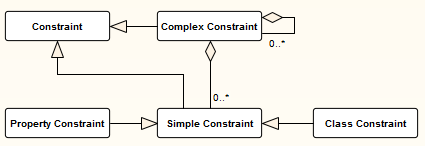
\includegraphics[width=0.80\textwidth]{images/RDF-CV-conceptual-model.png}
	\caption{\emph{RDF Constraints Vocabulary (RDF-CV)} - conceptual model}
	\label{fig:RDF-CV-conceptual-model}
\end{figure}

Constraints can be expressed either generically (\textbf{\emph{generic constraints}}) by the \emph{RDF-CV}   
or specifically (\textbf{\emph{specific constraints}}) by domain-specific constraint languages.
As the \emph{RDF-CV} describes constraints generically, the vocabulary does not distinguish constraints according to the dimension \emph{universality}. 
The majority of the constraint types can be expressed in \emph{DL}.
In contrast, there are constraint types which cannot be expressed in \emph{DL}, but are also representable by the \emph{RDF-CV} (see section \ref{sec:evaluation}). 
\textbf{\emph{Complex constraints}} encompass \textbf{\emph{simple constraints}} (atomic constraints) and/or further \emph{complex constraints},
i.e. \emph{DL} statements representing \emph{complex constraints} are created out of \emph{DL} statements standing for atomic and composed constraints (if expressible in \emph{DL}). 
Simple constraints may be applied to either properties (\textbf{\emph{property constraints}}) or classes (\textbf{\emph{class constraints}}).
The \emph{RDF-CV} does not contain any terms standing for \emph{simple} and \emph{complex constraints}, since \emph{context classes} of \emph{simple constraints} are just reused within \emph{complex constraints} (\emph{simple constraints} associated with \emph{context classes} must hold for individuals of these \emph{context classes}).
As a consequence, the distinction of \emph{property} and \emph{class constraints} is sufficient to describe constraints of all possible constraint types.

\subsection{\emph{Simple Constraints} (Expressible in \emph{DL})}

Sub-classes of \textbf{\emph{simple constraints}} are \textbf{\emph{property constraints}} and \textbf{\emph{class constraints}} (see the \emph{RDF-CV} implementation model in figure \ref{fig:RDF-CV-implementation-model}). 
For both \emph{property} and \emph{class constraints} a \emph{context class}, a list of \emph{classes}, the \emph{constraining element}, and the \emph{constraining value} can be stated. 
Lists of \emph{left} and \emph{right properties} can only be specified for \emph{property constraints}.

\begin{figure}
	\centering
		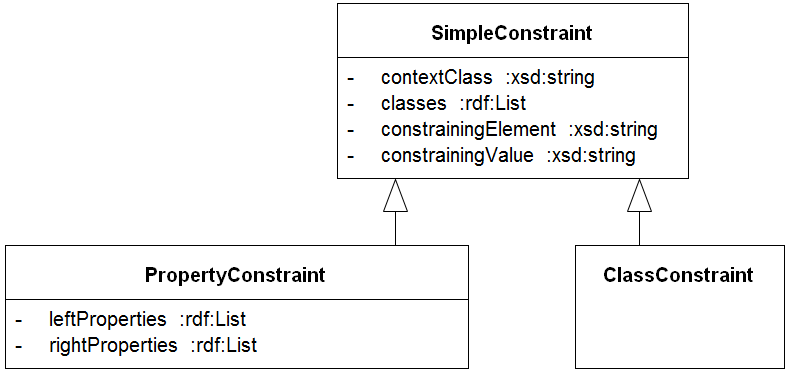
\includegraphics[width=0.70\textwidth]{images/RDF-CV-implementation-model.png}
	\caption{\emph{RDF Constraints Vocabulary (RDF-CV)} - implementation model}
	\label{fig:RDF-CV-implementation-model}
\end{figure}

A \emph{simple constraint} holds for all individuals of a \textbf{\emph{context class}}.
Consider, e.g., the following \emph{minimum qualified cardinality restriction} on the object property \emph{author}, which restricts \emph{publications} to have at least one \emph{author} which is a \emph{person}: 
\begin{DL}
$Publication \sqsubseteq \geq1 author . Person $
\end{DL}
The cardinality restriction is a constraint on the property \emph{author} and is therefore classified as a \emph{property constraint} which holds for all individuals of the class \emph{Publication} (see table \ref{tab:property-constraint-cardinality-restriction} for the mapping to \emph{RDF-CV}):

\begin{table}
  \scriptsize
  \sffamily
  \vspace{0cm}
	\centering
		\begin{tabular}{l|l|l|l|l|l|l}
      \textbf{c. type} & \textbf{context class} & \textbf{left p. list} & \textbf{right p. list} & \textbf{classes} & \textbf{c. element} & \textbf{c. value} \\
      \hline
      property & Publication & author & - & Person & $\geq$ & 1 \\
		\end{tabular}
	\caption{Property Constraint - Cardinality Restriction}
	\label{tab:property-constraint-cardinality-restriction}
\end{table}

The \textbf{\emph{constraining element}} indicates the actual type of constraint like \emph{DL} concept and role constructors, (in)equality, and further keywords for constraint types which cannot be expressed in \emph{DL} (e.g. regular expressions and constraining facets).
In some cases, a constraint is only complete when in addition to the \emph{constraining element} a \textbf{\emph{constraining value}} is stated.
The cardinality restriction 
\ms{$\geq$1 author.Person}, e.g., 
constructs an anonymous class of all individuals having at least one \emph{author} relationship to \emph{persons}.
The \emph{constraining element} of this \emph{property constraint} is the \emph{DL} at-least restriction \emph{$\geq$} and the \emph{constraining value} is \emph{1}.
\emph{Simple constraints} may refer to a list of \textbf{\emph{classes}}.
The qualified cardinality restriction above, e.g., refers to the class \emph{Person}, 
i.e. restricts the objects of the property \emph{author} to be of the class \emph{Person}.

For \emph{property constraints}, \textbf{\emph{left}} and \textbf{\emph{right property lists}} are specified.
The assignment of properties to these lists happens relative to the \emph{constraining element} - which may be an operator (e.g., $\sqsubseteq$ in case of \emph{object property paths}).
\emph{Object Property Paths} (\emph{R-55}; also called \emph{complex role inclusion axioms} in \emph{DL})
express that, if an individual \emph{x} is connected by a sequence of object properties with an individual \emph{y}, 
then \emph{x} is also related to \emph{y} by a particular object property. 
As \emph{Stephen-Hawking} is the \emph{author} of the book \emph{A-Brief-History-Of-Time} (\ms{authorOf(Stephen-Hawking, A-Brief-History-Of-Time)}) whose \emph{genre} is \emph{Popular-Science} ({\ms{genre(A-Brief-History-Of-Time, Popular-Science)}),
the following \emph{object property path} infers that \emph{Stephen-Hawking} is an \emph{author} of the \emph{genre} \emph{Popular-Science} (\ms{authorOfGenre(Stephen-Hawking, Popular-Science)}):
\begin{DL}
authorOf $\circ$ genre $\sqsubseteq$ authorOfGenre 
\end{DL}
Thus, when mapped to the \emph{RDF-CV} (see table \ref{tab:property-constraint-object-property-paths}), the properties \emph{authorOf} and \emph{genre} are on the left side of the \emph{constraining element} \emph{$\sqsubseteq$},
and the property \emph{authorOfGenre} is on the right side:

\begin{table}
  \scriptsize
  \sffamily
  \vspace{0cm}
	\centering
		\begin{tabular}{l|l|l|l|l|l|l}
      \textbf{c. type} & \textbf{context class} & \textbf{left p. list} & \textbf{right p. list} & \textbf{classes} & \textbf{c. element} & \textbf{c. value} \\
      \hline
      property & $\top$ & authorOf, genre & authorOfGenre & $\top$ & $\sqsubseteq$ & - \\
		\end{tabular}
	\caption{Property Constraint - Object Property Paths}
	\label{tab:property-constraint-object-property-paths}
\end{table}

\subsection{\emph{Simple Constraints} (Not Expressible in \emph{DL})}

There are \emph{simple constraints} which cannot be expressed in \emph{DL} such as \emph{literal pattern matching}, \emph{literal value comparison}, \emph{literal ranges}, \emph{default values}, and \emph{language tag cardinality} \cite{BoschNolleAcarEckert2015}.
% maybe additional constraint default values:
% ear shape of races, e.g. vulcans / teeth color
% mathematical operations

{\em Literal pattern matching} (\emph{R-44}) restricts literals to match given patterns.
The following \emph{universal restriction}, e.g., ensures that \emph{books} can only have valid \emph{ISBN} identifiers, 
i.e., strings that match a given regular expression:
\begin{DL}
\ms{Book $\sqsubseteq$ $\forall$ identifier.ISBN} 
\end{DL}
Even though, the restriction of the datatype \emph{ISBN} cannot be expressed in \emph{DL}, \emph{OWL 2 DL} can be used to express the \emph{literal pattern matching} constraint:

\begin{ex}
ISBN a RDFS:Datatype ; owl:equivalentClass [ a RDFS:Datatype ;
    owl:onDatatype xsd:string ; 
    owl:withRestrictions ([ xsd:pattern "^\d{9}[\d|X]$" ])] .
\end{ex}\$$
The first OWL 2 axiom explicitly declares {\em ISBN} to be a datatype. %\er{Why start from second and then first? Also better we say "owl axiom" when we talk axiom of owl, to prevent ambiguity.}\tb{resolved}
The second OWL 2 axiom defines {\em ISBN} as an abbreviation for a datatype restriction on {\em xsd:string}. 
The datatype {\em ISBN} can be used just like any other datatype like in the \emph{universal restriction} above.
%There are multiple use cases associated with the requirement to match literals according to given patterns (\emph{Literal Pattern Matching}\footnote{Corresponds to \emph{R-44-PATTERN-MATCHING-ON-RDF-LITERALS}}).
%The enterprise vessel, e.g.,  can only have the registry numbers "NCC-1701", "NCC-1701-A", "NCC-1701-B", "NCC-1701-C", "NCC-1701-D", or "NCC-1701-E".
%The universal restriction can be represented in DL:
%\ms{Enterprise $\sqsubseteq$ $\forall$ registryNumber.RegistryNumber}.
%The restriction of the datatype \ms{RegistryNumber}, however, cannot be expressed in DL, but OWL 2 DL can be used anyway to express the literal pattern matching constraint:
%
%\begin{ex}
%RegistryNumber
    %a rdfs:Datatype ; owl:equivalentClass [ a rdfs:Datatype ;
        %owl:onDatatype xsd:string ;
        %owl:withRestrictions ( [ xsd:pattern "NCC-1701([-][A-E])?" ] ) ] .
%\end{ex}
%The second axiom defines \ms{RegistryNumber} as an abbreviation for a datatype restriction on \ms{xsd:string}. 
%The first axiom explicitly declares \ms{RegistryNumber} to be a datatype. 
%The datatype \ms{RegistryNumber} can be used just like any other datatype like in the universal restriction above.
The \emph{literal pattern matching} constraint validates \emph{ISBN} literals according to the regular expression causing constraint violations for triples which do not not match. 
%\ms{Janeway commandsEnterprise Voyager} and \ms{Voyager registryNumber "NCC-74656"\textasciicircum{}\textasciicircum{}RegistryNumber}, 
%but not for the triples \ms{Picard commandsEnterprise Enterprise} and \ms{Enterprise registryNumber "NCC-1701-E"\textasciicircum{}\textasciicircum{}RegistryNumber}.
In table \ref{tab:simple-constraint-not-expressible-in-dl)}, the \emph{simple constraint} (\emph{literal pattern matching}) and the \emph{complex constraint} (\emph{universal restriction}) are mapped to the \emph{RDF-CV}:

%\begin{gcotable}
%property & Enterprise & registryNumber & - & RegistryNumber & $\forall$ & - \\
%class & RegistryNumber & - & - & xsd:string & regex & 'NCC-1701([-][A-E])?' \\
%\end{gcotable}

\begin{table}
  \scriptsize
  \sffamily
  \vspace{0cm}
	\centering
		\begin{tabular}{l|l|l|l|l|l|l}
      \textbf{c. type} & \textbf{context class} & \textbf{left p. list} & \textbf{right p. list} & \textbf{classes} & \textbf{c. element} & \textbf{c. value} \\
      \hline
      property & Book & identifier & - & ISBN & $\forall$ & - \\
      class & ISBN & - & - & xsd:string & regex & '\string^\text{$\backslash$d$\{9\}$[$\backslash$d$\mid$X]}\$' \\
		\end{tabular}
	\caption{Simple Constraint (Not Expressible in DL)}
	\label{tab:simple-constraint-not-expressible-in-dl)}
\end{table} %\tb{Erman, can you please format the regular expression in the table above correctly?}
The \emph{literal pattern matching} constraint type introduces the new \emph{constraining element} \emph{regex},
for which a validation mechanism has to be implemented.
Validation has to be implemented once for each \emph{generic constraint type} which is not expressible in \emph{DL}.

\subsection{\emph{Complex Constraints}}

\textbf{\emph{Complex constraints}} are composed out of \emph{simple constraints} and/or \emph{complex constraints}.
\emph{Exclusive or} is a logical operation that outputs true whenever both inputs differ (one is true, the other is false).
The \emph{complex constraint} \emph{context-specific exclusive or of property groups} (\emph{R-13})
restricts individuals of given classes to have properties of only one of multiple mutually exclusive property groups.
\emph{Publications}, e.g., are either identified by an \emph{ISBN} and a \emph{title} (for books) or by an \emph{ISSN} and a \emph{title} (for periodical \emph{publications}), but it should not be possible to assign both identifiers to a given \emph{publication}, which can be expressed in \emph{ShEx} as follows:

%Half-Klingons, e.g., either have a klingon mother and a human father or a human mother and a klingon father, which can be expressed by ShEx:

%\begin{ex}
%Half-Klingon { 
    %( klingonMother Klingon , humanFather Human ) |
    %( humanMother Human , klingonFather Klingon ) }
%\end{ex}

\begin{ex}
Publication { 
    ( isbn string , title string ) |
    ( issn string , title string ) }
\end{ex}

%As \ms{B'Elanna Torres} is a \ms{Half-Klingon} with a klingon mother and a human father, the following data is valid:

%\begin{ex}
%BElannaTorres a Half-Klingon ;
    %klingonMother Miral ; humanFather JohnTorres .
%\end{ex}

As the \emph{The-Great-Gatsby} is a \emph{publication} (\ms{rdf:type(The-Great-Gatsby, Publication)}) having an \emph{ISBN} number (\ms{isbn(The-Great-Gatsby, '978-0241965672')}) and a \emph{title} (\ms{title(The-Great-Gatsby, 'The Great Gatsby')}) and not an additional \emph{ISSN} identifier, the \emph{The-Great-Gatsby} is a valid \emph{publication}.
%\begin{DL}
%rdf:type(BElannaTorres,Half-Klingon) \\
%klingonMother(BElannaTorres,Miral) \\
%klingonMother(BElannaTorres,JohnTorres)
%\end{DL}
The \emph{complex constraint} is mapped to the \emph{RDF-CV} (see table \ref{tab:complex-constraints}) and expressed in \emph{DL} as follows:

%\begin{DL}
%Half-Klingon $\sqsubseteq$ ($\neg$E $\sqcap$ F) $\sqcup$ (E $\sqcap$ $\neg$F) \\ 
%E $\equiv$ A $\sqcap$ B \\
%F $\equiv$ C $\sqcap$ D \\
%A $\sqsubseteq$ $\geq$ 1 klingonMother.Klingon $\sqcap$ $\leq$ 1 klingonMother.Klingon \\
%B $\sqsubseteq$ $\geq$ 1 humanFather.Human $\sqcap$ $\leq$ 1 humanFather.Human \\
%C $\sqsubseteq$ $\geq$ 1 humanMother.Human $\sqcap$ $\leq$ 1 humanMother.Human \\
%D $\sqsubseteq$ $\geq$ 1 klingonFather.Klingon $\sqcap$ $\leq$ 1 klingonFather.Klingon \\
%\end{DL}

\begin{DL}
Publication $\sqsubseteq$ ($\neg$E $\sqcap$ F) $\sqcup$ (E $\sqcap$ $\neg$F) \\ 
E $\equiv$ A $\sqcap$ B \\
F $\equiv$ C $\sqcap$ D \\
A $\sqsubseteq$ $\geq$ 1 isbn.string $\sqcap$ $\leq$ 1 isbn.string \\
B $\sqsubseteq$ $\geq$ 1 title.string $\sqcap$ $\leq$ 1 title.string \\
C $\sqsubseteq$ $\geq$ 1 issn.string $\sqcap$ $\leq$ 1 issn.string \\
D $\sqsubseteq$ $\geq$ 1 title.string $\sqcap$ $\leq$ 1 title.string \\
\end{DL}

%\begin{gcotable}
%class & Half-Klingon & - & - & $\neg$E $\sqcap$ F, E $\sqcap$ $\neg$F & $\sqcup$ & - \\
%class & $\neg$E $\sqcap$ F & - & - & $\neg$E, F & $\sqcap$ & - \\
%class & E $\sqcap$ $\neg$F & - & - & E, $\neg$F & $\sqcap$ & - \\
%class & $\neg$E & - & - & E & $\neg$ & - \\
%class & E & - & - & A, B & $\sqcap$ & - \\
%class & $\neg$F & - & - & F & $\neg$ & - \\
%class & F & - & - & C, D & $\sqcap$ & - \\
%class & A & - & - & A1, A2 & $\sqcap$ & - \\
%property & A1 & klingonMother & - & Klingon & $\geq$ & 1 \\
%property & A2 & klingonMother & - & Klingon & $\leq$ & 1 \\
%class & B & - & - & B1, B2 & $\sqcap$ & - \\
%property & B1 & humanFather & - & Human & $\geq$ & 1 \\
%property & B2 & humanFather & - & Human & $\leq$ & 1 \\
%class & C & - & - & C1, C2 & $\sqcap$ & - \\
%property & C1 & humanMother & - & Human & $\geq$ & 1 \\
%property & C2 & humanMother & - & Human & $\leq$ & 1 \\
%class & D & - & - & D1, D2 & $\sqcap$ & - \\
%property & D1 & klingonFather & - & Klingon & $\geq$ & 1 \\
%property & D2 & klingonFather & - & Klingon & $\leq$ & 1 \\
%\end{gcotable}

\begin{table}
  \scriptsize
  \sffamily
  \vspace{0cm}
	\centering
		\begin{tabular}{l|l|l|l|l|l|l}
      \textbf{c. type} & \textbf{context class} & \textbf{left p. list} & \textbf{right p. list} & \textbf{classes} & \textbf{c. element} & \textbf{c. value} \\
      \hline
class & Publication & - & - & $\neg$E $\sqcap$ F, E $\sqcap$ $\neg$F & $\sqcup$ & - \\
class & $\neg$E $\sqcap$ F & - & - & $\neg$E, F & $\sqcap$ & - \\
class & E $\sqcap$ $\neg$F & - & - & E, $\neg$F & $\sqcap$ & - \\
class & $\neg$E & - & - & E & $\neg$ & - \\
class & E & - & - & A, B & $\sqcap$ & - \\
class & $\neg$F & - & - & F & $\neg$ & - \\
class & F & - & - & C, D & $\sqcap$ & - \\
class & A & - & - & A1, A2 & $\sqcap$ & - \\
property & A1 & isbn & - & string & $\geq$ & 1 \\
property & A2 & isbn & - & string & $\leq$ & 1 \\
class & B & - & - & B1, B2 & $\sqcap$ & - \\
property & B1 & title & - & string & $\geq$ & 1 \\
property & B2 & title & - & string & $\leq$ & 1 \\
class & C & - & - & C1, C2 & $\sqcap$ & - \\
property & C1 & issn & - & string & $\geq$ & 1 \\
property & C2 & issn & - & string & $\leq$ & 1 \\
class & D & - & - & D1, D2 & $\sqcap$ & - \\
property & D1 & title & - & string & $\geq$ & 1 \\
property & D2 & title & - & string & $\leq$ & 1 \\
		\end{tabular}
	\caption{Complex Constraints}
	\label{tab:complex-constraints}
\end{table}

%Even though, tools may generate \emph{generic constraints} automatically, this 
\emph{Complex constraints} are composed of many other \emph{complex} (e.g. \emph{minimum and maximum qualified cardinality restrictions}) and \emph{simple constraints} (e.g. constraints on sets).
As \emph{exact (un)qualified cardinality restrictions (=n)} and \emph{exclusive or (XOR)} are frequently used \emph{complex constraints},
we propose using them as \emph{simple constraints} - in terms of syntactic sugar.
As a consequence, the \emph{context-specific exclusive or of property groups} constraint above is represented as a \emph{generic constraint} more intuitively and concisely (see table \ref{tab:simplified-complex-constraints}).

%\begin{gcotable}
%class & Half-Klingon & - & - & E, F & XOR \\
%class & E & - & - & A, B & $\sqcap$ \\
%class & F & - & - & C, D & $\sqcap$ \\
%property & A & klingonMother & - & Klingon & = & 1 \\
%property & B & humanFather & - & Human & = & 1 \\
%property & C & humanMother & - & Human & = & 1 \\
%property & D & klingonFather & - & Klingon & = & 1 \\
%\end{gcotable}

\begin{table}
  \scriptsize
  \sffamily
  \vspace{0cm}
	\centering
		\begin{tabular}{l|l|l|l|l|l|l}
      \textbf{c. type} & \textbf{context class} & \textbf{left p. list} & \textbf{right p. list} & \textbf{classes} & \textbf{c. element} & \textbf{c. value} \\
      \hline
class & Publication & - & - & E, F & XOR \\
class & E & - & - & A, B & $\sqcap$ \\
class & F & - & - & C, D & $\sqcap$ \\
property & A & isbn & - & string & = & 1 \\
property & B & title & - & string & = & 1 \\
property & C & issn & - & string & = & 1 \\
property & D & title & - & string & = & 1 \\
		\end{tabular}
	\caption{Simplified Complex Constraints}
	\label{tab:simplified-complex-constraints}
\end{table}

\subsection{\emph{Complex Constraints} as \emph{Simple Constraints}}

Almost 15 percent of all constraint types are \emph{complex constraints} which can be simplified and therefore formulated as \emph{simple constraints} when using them in terms of syntactic sugar (see section \ref{sec:evaluation}).

There are three forms of \emph{OWL RBox axioms}: \emph{role inclusions}, \emph{equivalence} and \emph{disjointness}. 
\emph{OWL} provides a variety of other axiom types: \emph{role transitivity}, \emph{symmetry}, \emph{asymmetry}, \emph{reflexivity} and \emph{irreflexivity}. 
These axiom types are sometimes considered as basic axiom types in \emph{DL} - using some suggestive notation such as
\ms{Trans(ancestorOf)} to express that the role \emph{ancestorOf} is transitive.
Such axioms, however, are just syntactic sugar - 
all role characteristics can be expressed using the basic features of \emph{DL}.
The \emph{irreflexive object properties} constraint type (\emph{R-60}) 
restricts that no individual is connected by a given object property to itself \cite{Kroetzsch2012}.
With the following \emph{irreflexive object property} constraint, e.g., one can state that individuals cannot be authors of themselves:
\begin{DL}
\ms{$\top$ $\sqsubseteq$ $\neg$ $\exists authorOf.Self$}
\end{DL}
When mapped to the \emph{RDF-CV} (see table \ref{tab:irreflexive-object-properties-as-complex-constraints}), the \emph{complex constraint} aggregates three \emph{simple constraints} (one \emph{property} and two \emph{class constraints}):

%\begin{gcotable}
%property & $\exists$ marriedTo . Self & marriedTo & - & Self & $\exists$ & - \\
%class & $\neg$ $\exists$ marriedTo . Self & - & - & $\exists$ marriedTo . Self & $\neg$ & - \\
%class & $\top$ & - & - & $\top$, $\neg$ $\exists$ marriedTo . Self & $\sqsubseteq$ & - \\
%\end{gcotable}

\begin{table}
  \scriptsize
  \sffamily
  \vspace{0cm}
	\centering
		\begin{tabular}{l|l|l|l|l|l|l}
      \textbf{c. type} & \textbf{context class} & \textbf{left p. list} & \textbf{right p. list} & \textbf{classes} & \textbf{c. element} & \textbf{c. value} \\
      \hline
property & $\exists$ authorOf.Self & marriedTo & - & Self & $\exists$ & - \\
class & $\neg$ $\exists$ authorOf.Self & - & - & $\exists$ authorOf.Self & $\neg$ & - \\
class & $\top$ & - & - & $\top$, $\neg$ $\exists$ authorOf.Self & $\sqsubseteq$ & - \\
		\end{tabular}
	\caption{Irreflexive Object Properties as Complex Constraints}
	\label{tab:irreflexive-object-properties-as-complex-constraints}
\end{table}

When using the \emph{OWL RBox axiom} \emph{role irreflexivity} in terms of syntactic sugar, 
the \emph{complex constraint} can be expressed more concisely in form of a \emph{simple property constraint} with exactly the same semantics (see table \ref{tab:irreflexive-object-properties-as-simple-constraints}):

%\begin{gcotable}
%property & $\top$ & marriedTo & - & - & irreflexive & - \\
%\end{gcotable}

\begin{table}
  \scriptsize
  \sffamily
  \vspace{0cm}
	\centering
		\begin{tabular}{l|l|l|l|l|l|l}
      \textbf{c. type} & \textbf{context class} & \textbf{left p. list} & \textbf{right p. list} & \textbf{classes} & \textbf{c. element} & \textbf{c. value} \\
      \hline
property & $\top$ & authorOf & - & - & irreflexive & - \\
		\end{tabular}
	\caption{Irreflexive Object Properties as Simple Constraints}
	\label{tab:irreflexive-object-properties-as-simple-constraints}
\end{table}

The \emph{primary key properties} constraint type (\emph{R-226}) is often useful to declare a given (datatype) property as the "primary key" of a class, so that a system can enforce uniqueness. 
\emph{Books}, e.g., are uniquely identified by their \emph{ISBN} number, i.e., the property \emph{isbn} is inverse functional \ms{$(\ms{funct } isbn\sp{\overline{\ }})$}, 
which can be represented by the \emph{RDF-CV} in form of a \emph{complex constraint} (see table \ref{tab:primary-key-properties-as-complex-constraints}):

%\begin{gcotable}
%property & $\top$ & commandAuthorizationCode$^{-}$ & commandAuthorizationCode$^{-}$ & - & inverse & - \\
%property & $\top$ & commandAuthorizationCode$^{-}$ & - & - & functional & - \\
%\end{gcotable}

\begin{table}
  \scriptsize
  \sffamily
  \vspace{0cm}
	\centering
		\begin{tabular}{l|l|l|l|l|l|l}
      \textbf{c. type} & \textbf{context class} & \textbf{left p. list} & \textbf{right p. list} & \textbf{classes} & \textbf{c. element} & \textbf{c. value} \\
      \hline
property & $\top$ & isbn$^{-}$ & isbn$^{-}$ & - & inverse & - \\
property & Book & isbn$^{-}$ & - & - & functional & - \\
		\end{tabular}
	\caption{Primary Key Properties as Complex Constraints}
	\label{tab:primary-key-properties-as-complex-constraints}
\end{table}

\emph{Keys}, however, are even more general, i.e., a generalization of \emph{inverse functional properties} \cite{Schneider2009}.
A key can be a datatype, an object property, or a chain of properties.
For these generalization purposes, as there are different sorts of keys, and as keys can lead to undecidability, 
\emph{DL} is extended with \emph{key boxes} and a special construct \emph{keyfor} \cite{Lutz2005}.
When using the \emph{keyfor} \emph{DL} construct (\ms{isbn keyfor Book}), the \emph{complex constraint} can be expressed by only one \emph{simple property constraint} (see table \ref{tab:primary-key-properties-as-simple-constraints} for the mapping to the \emph{RDF-CV}).

%\begin{gcotable}
%property & StarFleetOfficer & commandAuthorizationCode & - & - & keyfor & - \\
%\end{gcotable}

\begin{table}
  \scriptsize
  \sffamily
  \vspace{0cm}
	\centering
		\begin{tabular}{l|l|l|l|l|l|l}
      \textbf{c. type} & \textbf{context class} & \textbf{left p. list} & \textbf{right p. list} & \textbf{classes} & \textbf{c. element} & \textbf{c. value} \\
      \hline
property & Book & isbn & - & - & keyfor & - \\
		\end{tabular}
	\caption{Primary Key Properties as Simple Constraints}
	\label{tab:primary-key-properties-as-simple-constraints}
\end{table}

%Starfleet officers, e.g., are uniquely identified by their command authorization code (e.g. to activate and cancel auto-destruct sequences).
%It means that the property \emph{commandAuthorizationCode} is inverse functional - mapped to DL and the \emph{RDF-CV} as follows:
%
%\begin{DL}
%$(\ms{funct } commandAuthorizationCode\sp{\overline{\ }})$
%\end{DL}
%
%%\begin{gcotable}
%%property & $\top$ & commandAuthorizationCode$^{-}$ & commandAuthorizationCode$^{-}$ & - & inverse & - \\
%%property & $\top$ & commandAuthorizationCode$^{-}$ & - & - & functional & - \\
%%\end{gcotable}
%
%\begin{table}
  %\scriptsize
  %\sffamily
  %\vspace{0cm}
	%\centering
		%\begin{tabular}{l|l|l|l|l|l|l}
      %\textbf{c. type} & \textbf{context class} & \textbf{left p. list} & \textbf{right p. list} & \textbf{classes} & \textbf{c. element} & \textbf{c. value} \\
      %\hline
%property & $\top$ & commandAuthorizationCode$^{-}$ & commandAuthorizationCode$^{-}$ & - & inverse & - \\
%property & $\top$ & commandAuthorizationCode$^{-}$ & - & - & functional & - \\
		%\end{tabular}
	%\caption{Primary Key Properties as Complex Constraints}
	%\label{tab:primary-key-properties-as-complex-constraints}
%\end{table}
%
%Keys, however, are even more general, i.e., a generalization of inverse functional properties \cite{Schneider2009}.
%A key can be a datatype property, an object property, or a chain of properties.
%For this generalization purposes, as there are different sorts of key, and as keys can lead to undecidability, 
%DL is extended with \emph{key boxes} and a special \emph{keyfor} construct\cite{Lutz2005}.
%This leads to the following DL and \emph{RDF-CV} mappings (only one \emph{simple property constraint}):
%
%\begin{DL}
%commandAuthorizationCode \ms{keyfor} StarfleetOfficer
%\end{DL}

%\begin{table}
  %\scriptsize
  %\sffamily
  %\vspace{0cm}
	%\centering
		%\begin{tabular}{l|l|l|l|l|l|l}
      %\textbf{c. type} & \textbf{context class} & \textbf{left p. list} & \textbf{right p. list} & \textbf{classes} & \textbf{c. element} & \textbf{c. value} \\
      %\hline
%property & StarFleetOfficer & commandAuthorizationCode & - & - & keyfor & - \\
		%\end{tabular}
	%\caption{Primary Key Properties as Simple Constraints}
	%\label{tab:primary-key-properties-as-simple-constraints}
%\end{table}

%\begin{itemize}
  %\item domain and range
	%\item Primary Key Properties
	%\item ( Exact Qualified Cardinality Restrictions on Properties )
%\end{itemize}

%\subsection{Disjoint Classes}
%
%\begin{DL}
%Hologram $\sqcap$ Human $\sqsubseteq$ $\perp$\\
%Alternative:\\
%$Hologram \sqsubseteq \neg Human$
%\end{DL}
%
%\subsection{Minimum Qualified Cardinality Restrictions on Properties}
%
%\begin{DL}
%$FederationCaptain \sqsubseteq Federation \sqcap \geq1 commandsVessel . Vessel $
%\end{DL}

%\section{Transformations and Automatic Validation of Specific Constraints}
%\section{Transformations between Specific Constraints (Expressed by Different Constraint Languages)}
%\section{Transformations between Specific Constraints}
\section{How to Improve the Understandability of Constraints}
\label{sec:transformations}

RDF data providers have to ensure that their data conforms to constraints which are explicitly defined within contracts between data providers and consumers.
As there is no standard way to express constraints, they may be represented by a variety of constraint languages\footnote{Candidates for constraint languages are, i.a., SPIN, OWL 2, DSP, ShEx, ReSh, Bibframe, DQTP, Pellet ICV, RDFUnit, SPARQL, and Stardog ICV} - each of them different in syntax and semantics.
To overcome the necessity to understand diverse constraint languages, 
we propose to transform any \emph{specific constraint} (\emph{$sc_{\alpha}$}) (expressed by any constraint language \emph{$\alpha$}) into any other \emph{specific constraint} (\emph{$sc_{\beta}$}) (expressed by any other constraint language \emph{$\beta$}) - in case they have the same semantics.
We use the \emph{RDF-CV} to intermediately represent constraints in a generic way for these transformations.
By defining mappings ($m(sc_{\alpha}), m(sc_{\beta})$) between equivalent \emph{specific constraints} and the corresponding \emph{generic constraint} (\emph{gc}) we are able to convert them automatically:

\begin{DL}
$ gc = m(sc_{\alpha}) = m(sc_{\beta}) $
\end{DL}

We do not need to define mappings between each pair of semantically equivalent \emph{specific constraints}.
Let's assume we are able to express a particular constraint type by 5/6/7/8/9/10 constraint languages.
Without the intermediate \emph{generic constraint}, we would have to define for each constraint type \emph{1} mapping for each pair of \emph{specific constraints} (expressed by different constraint languages)
- that are \emph{\( {n \choose 2} \)} mappings (10/15/21/28/36/45 mappings).
With an intermediate \emph{generic constraint}, however, we only need to define for each constraint type \emph{n} mappings (1 mapping for each \emph{specific constraint}) from \emph{n} \emph{specific constraints} to the corresponding \emph{generic constraint} (5/6/7/8/9/10 mappings).

%(n(n+1))/2

%\begin{DL}
%\(\sum \limits_{i=1}^n i = \frac{n(n+1)}{2}\)
%\(\sum \limits_{i=1}^n i\)
%\(\Binom{n}{2} \)
%\( {n \choose 2} \)
%\end{DL}

\begin{DL}
Publication $\equiv$ $\exists$ publisher.Publisher
\end{DL}

The {\em existential quantification} (\emph{R-86})
%\ms{Publication $\equiv$ $\exists$ publisher.Publisher} 
above restricts \emph{publications} to have at least one \emph{publisher} and can be expressed by at least 10 different constraint languages\footnote{OWL 2, SPARQL, ShEx, Bibframe, DSP, ReSh, SPIN, DQTP, Pellet IVC, and Stardog ICV}:

\begin{ex}
# OWL 2:
[ a owl:Restriction ;
  owl:onProperty publisher ;
  owl:someValuesFrom Publisher ;
  rdfs:subClassOf Publication ] .
	
# SPARQL:
ASK { ?x a Publication . FILTER NOT EXISTS { ?x publisher [ a Publisher ] } . }
	
# ShEx:
Publication {
    publisher @Publisher{1,} }
		
# DSP:
descriptionTemplate a dsp:DescriptionTemplate ;
    dsp:resourceClass Publication ; 
    dsp:statementTemplate [ a dsp:NonLiteralStatementTemplate ;
        dsp:minOccur 1 ; dsp:maxOccur "infinity" ; 
        dsp:property publisher ; 
        dsp:nonLiteralConstraint [ a dsp:NonLiteralConstraint ;
            dsp:valueClass Publisher ] ] .
		
# ReSh:
Publication a rs:ResourceShape ; rs:property [
    rs:propertyDefinition :publisher ;
    rs:valueShape :Publisher ;
    se:min 1 ; se:maxundefined true ; ] .
		
# SPIN:
CONSTRUCT {
    _:cv a spin:ConstraintViolation ; spin:violationRoot ?subject ;
         rdfs:label ?violationMessage ; spin:violationPath ?property . } WHERE 
{ ?subject a ?classSubject . FILTER NOT EXISTS { ?subject ?property [ a ?classObject ] } . }
\end{ex}

%\emph{Allowed Values}\footnote{corresponds to \emph{R-30-ALLOWED-VALUES-FOR-RDF-OBJECTS} and \emph{R-37-ALLOWED-VALUES-FOR-RDF-LITERALS}}
%is a common requirement (constraint type) to narrow down the value space of a property by an exhaustive enumeration of the valid values (both literals or resources). 
%The Enterprise, e.g., is only commanded by the captains Archer, Kirk, and Picard.
%This \emph{complex constraint} is composed of the two \emph{simple constraints} \emph{universal quantification} and \emph{allowed values} which can be represented in DL:

%\begin{DL}
%StarfleetCaptain $\equiv$ $\forall$ overruledBy . \{Commodore\} $\sqcup$ \{Admiral\}
%\end{DL}

%\begin{DL}
%Enterprise $\equiv$ $\forall$ commandedBy . \{Archer\} $\sqcup$ \{Kirk\} $\sqcup$ \{Picard\}
%\end{DL}

%First, we map these DL statements to two \emph{simple generic constraints} corresponding to the \emph{RDF-CV} (we define the class \ms{EnterpriseCaptains} by simply enumerating its instances):

The \emph{DL} statement \ms{Publication $\equiv$ $\exists$ publisher.Publisher} is mapped to a \emph{(simple) generic constraint} conforming to the \emph{RDF-CV} (see table \ref{tab:existential-quantification-as-simple-constraints}).
Then, one mapping (\emph{$m(sc_{OWL 2})$}, \emph{$m(sc_{ReSh})$}, \emph{$m(sc_{ShEx})$}, ...) is defined for each \emph{specific constraint} (\emph{$sc_{OWL 2}$}, \emph{$sc_{ReSh}$}, \emph{$sc_{ShEx}$}, ...) to the corresponding \emph{generic constraint} (\emph{gc}).

%\begin{gcotable}
%property & StarfleetCaptain & overruledBy & - & CaptainOverruler & $\forall$ & - \\
%class & CaptainOverruler & - & - & \{Commodore\},\{Admiral\} & $\sqcup$ & - \\
%\end{gcotable}

%\begin{gcotable}
%property & Enterprise & commandedBy & - & EnterpriseCaptains & $\forall$ & - \\
%class & EnterpriseCaptains & - & - & \{Archer\},\{Kirk\},\{Picard\} & $\sqcup$ & - \\
%\end{gcotable}

\begin{table}
  \scriptsize
  \sffamily
  \vspace{0cm}
	\centering
		\begin{tabular}{l|l|l|l|l|l|l}
      \textbf{c. type} & \textbf{context class} & \textbf{left p. list} & \textbf{right p. list} & \textbf{classes} & \textbf{c. element} & \textbf{c. value} \\
      \hline
property & Publication & publisher & - & Publisher & $\exists$ \\
		\end{tabular}
	\caption{Existential Quantification as Simple Constraints}
	\label{tab:existential-quantification-as-simple-constraints}
\end{table}

%\begin{ex}
%# OWL 2:
%Enterprise rdfs:subClassOf [ a owl:Restriction .
    %owl:onProperty commandedBy .
    %owl:allValuesFrom [ a owl:Class ;
        %owl:oneOf ( Archer Kirk Picard ) ] ] .
%# ReSh:
%Enterprise a rs:ResourceShape ; rs:property [
    %rs:name "commandedBy" ; rs:propertyDefinition commandedBy ;
    %rs:allowedValue Archer , Kirk , Picard ;
    %rs:occurs rs:Exactly-one ; ] .
%# ShEx:
%Enterprise {
    %commandedBy (Archer Kirk Picard) }
%\end{ex}

%\begin{ex}
%# DSP:
%[ a dsp:DescriptionTemplate ;
    %dsp:resourceClass StarfleetCaptain ; 
    %dsp:statementTemplate [ a dsp:NonLiteralStatementTemplate ; 
        %dsp:property overruledBy ; 
        %dsp:nonLiteralConstraint [ a dsp:NonLiteralConstraint ;
            %dsp:valueClass Commodore , Admiral ] ] ] .
%# OWL 2:
%StarfleetCaptain rdfs:subClassOf [ a owl:Restriction .
    %owl:onProperty overruledBy .
    %owl:allValuesFrom [ a owl:Class ;
        %owl:oneOf ( Commodore Admiral ) ] ] .
%# ReSh:
%%StarfleetCaptain a rs:ResourceShape ;
    %%rs:property [
        %%rs:name "overruledBy" ; rs:propertyDefinition overruledBy ;
        %%rs:valueShape Commodore ; rs:occurs rs:Zero-or-many ; ] ;
    %%rs:property [
        %%rs:name "overruledBy" ; rs:propertyDefinition overruledBy ;
        %%rs:valueShape Admiral ; rs:occurs rs:Zero-or-many ; ] ;
%# ShEx:
%:StarfleetCaptain {
    %:overruledBy @:Commodore* , :overruledBy @:Admiral* }
%\end{ex}

%\section{Validation of Specific and Generic Constraints}
\section{How to Provide Constraint Validation Out-Of-The-Box}
\label{sec:validation}

SPARQL is generally seen as the method of choice to validate RDF data according to certain constraints, although, it is not ideal for their formulation. 
In contrast, OWL 2, DSP, ReSh, and ShEx constraints are comparatively easy to understand. 
We use SPIN as basis to define a
validation environment in which the validation of any constraint language\footnote{The only limitation is that constraint languages must be represented in RDF} can be implemented by representing them in SPARQL
(the implementation can be tested at \url{http://purl.org/net/rdfval-demo}).
The SPIN engine checks for each resource if it satisfies all constraints, which are associated with the classes assigned to the resource, and generates a result RDF graph containing information about all constraint violations \cite{BoschEckert2014-2}.
This way, we are able to offer RDF data validation according to all \emph{specific constraints} (expressed by any constraint language) by defining mappings from each \emph{specific constraint} to \emph{SPIN}. 
We already specified mappings to \emph{SPIN} for all \emph{OWL 2} and \emph{DSP}\footnote{SPIN mappings: \url{https://github.com/boschthomas/rdf-validation/tree/master/SPIN}} constructs and for some \emph{ReSh} and \emph{ShEx} constructs.
%We do not have to define a mapping to SPIN for each specific constraint. 
%when we define a mapping to SPIN for each generic constraint.
As constraint languages differ in syntax and semantics it is rather difficult to ensure that semantically equivalent \emph{specific constraints} always lead to identical validation results.

We do not have to map each \emph{specific constraint} to SPIN and we get identical validation results for semantically equivalent \emph{specific constraints} (expressed by different constraint languages),
(1) if we map semantically equivalent \emph{specific constraints} to the corresponding \emph{generic constraint} and 
(2) if we map the \emph{generic constraint} to SPIN.
As a consequence, we only have to define one SPIN mapping for each constraint type corresponding to an RDF validation requirement.
19 of the overall 74 identified constraint types can be expressed by at least four constraint languages \cite{BoschNolleAcarEckert2015}.
This means that there must be 76 (four for each constraint type) implementations to validate RDF data according to 76 \emph{specific constraints} - instead of only 19 implementations (one for each \emph{generic constraint}) leading to identical validation results.

%The validation implementation of constraint languages is fully declarative,
%consisting of a mapping from constraint languages to SPIN in form of SPARQL CONSTRUCT queries.
%SPIN represents both the SPIN mappings and the SPARQL queries in RDF. 
%Within the validation environment, we fully implemented the validation of all OWL 2 DL and DSP constructs 
%(for the complete DSP validation see \cite{BoschEckert2014-2}). 

Within the \emph{RDF Validator}\footnote{For details about the validation environment see \cite{BoschEckert2014-2}}, we define one SPIN construct template for each \emph{generic constraint} and therefore constraint type.
A SPIN construct template contains a SPARQL CONSTRUCT query which generates constraint violation triples (\emph{spin:ConstraintViolation}) indicating the subject (\emph{spin:violationRoot}) and the properties (\emph{spin:violationPath}) causing constraint violations, and the reason why constraint violations have been raised (\emph{rdfs:label}).
A SPIN construct template creates constraint violation triples if all triple patterns within the SPARQL WHERE clause match.

\begin{DL}
Publication $\equiv$ $\forall$ author.Person
\end{DL}

According to the \emph{universal quantification} (\emph{R-91}) above, \emph{authors} of \emph{publications} must be \emph{persons}.
The SPARQL CONSTRUCT query for the constraint type \emph{universal quantification} is shown below:

\begin{ex}
CONSTRUCT {
    [   a spin:ConstraintViolation ; spin:violationRoot ?subject ;
        rdfs:label ?violationMessage ; spin:violationPath ?lp1 . ] }
WHERE {	  
    [   a gclo:PropertyConstraint ;
        gclo:contextClass ?cc ;
        gclo:leftProperties ( ?lp1 ) ;
        gclo:classes ( ?c1 ) ;
        gclo:constrainingElement "universal quantification" ] .
    ?subject a ?cc .
    ?subject ?lp1 ?o .
    FILTER NOT EXISTS { ?o a ?c1 } . }
\end{ex}

We provide a mapping from the \emph{RDF-CV} to SPIN\footnote{RDF-CV to SPIN: \url{https://github.com/boschthomas/RDF-CV-2-SPIN}} 
in order to automatically validate RDF data complying with each type of \emph{generic constraint} (\emph{simple}, \emph{complex}, \emph{property}, and \emph{class constraints}).

%\subsection{Not Allowed Values}

\section{Evaluation}
\label{sec:evaluation}

We evaluated to which extend the five most promising constraint languages on being the standard fulfill each of the overall 74 requirements to formulate RDF constraints; each of them corresponding to a constraint type.
We recently published a technical report\footnote{Available at: \url{http://arxiv.org/abs/1501.03933}} (serving as appendix of this paper) in which we explain each constraint type in detail and give examples for each (represented by different constraint languages).
The technical report also contains mappings to \emph{DL} to logically underpin each constraint type and to determine which \emph{DL} constructs are needed to express each constraint type \cite{BoschNolleAcarEckert2015}.
If a constraint type can be expressed in \emph{DL}, we added the mapping to \emph{DL} and to the \emph{generic constraint} conforming to the \emph{RDF-CV}.
In contrast, if a constraint type cannot be expressed in \emph{DL}, we only added the mapping to the \emph{generic constraint}.
This way, we prove that each constraint type can be mapped to a \emph{generic constraint} and therefore be represented generically by means of the \emph{RDF-CV}.
Table \ref{tab:evaluation} displays the classification of constraint types according to the dimensions \emph{context}, \emph{complexity}, and \emph{DL expressivity}:

%\begin{evaluation-generic-overview}
%\emph{Property Constraints} & 48 & 65 (64.86) \\
%\emph{Class Constraints} & 17 & 23 (22.96) \\
%\emph{Property and Class Constraints} & 9 & 12 (12.16) \\
%\hline
%\emph{Simple Constraints} & 46 & 62 (62.16) \\
%\emph{Simple Constraints} (Syntactic Sugar) & 10 & 14 (13.51) \\
%\emph{Complex Constraints} & 18 & 24 (24.32) \\
%\hline
%\emph{DL Expressible} & 51 & 69 (68.92) \\
%\emph{DL Not Expressible} & 23 & 31 (31.08) \\
%\hline
%Total & 74 & 100 \\
%\end{evaluation-generic-overview}

\begin{table}
  %\scriptsize
  %\sffamily
  \vspace{0cm}
	\centering
		\begin{tabular}{l|c|c}
      \textbf{Classes of Constraint Types} & \textbf{\#} & \textbf{\%} \\
      \hline
%\textbf{\emph{Context}} & & \\
\emph{Property Constraints} & 48 & 64.86 \\
\emph{Class Constraints} & 17 & 22.96 \\
\emph{Property and Class Constraints} & 9 & 12.16 \\
\hline
%\textbf{\emph{Complexity}} & & \\
\emph{Simple Constraints} & 46 & 62.16 \\
\emph{Simple Constraints} (Syntactic Sugar) & 10 & 13.51 \\
\emph{Complex Constraints} & 18 & 24.32 \\
\hline
%\textbf{\emph{DL Expressivity}} & & \\
\emph{DL Expressible} & 51 & 68.92 \\
\emph{DL Not Expressible} & 23 & 31.08 \\
\hline
Total & 74 & 100 \\
		\end{tabular}
	\caption{Evaluation}
	\label{tab:evaluation}
\end{table}

%\newenvironment{evaluation-generic-overview}{
  %%\scriptsize
  %%\sffamily
  %\vspace{0cm}
	%\begin{center}
  %\begin{tabular}{l|c|c}
  %\hline
  %\textbf{Constraint Classes} & \textbf{\#} & \textbf{\%} \\
  %\hline
%
%}{
  %\hline
  %\end{tabular}
  %%\linebreak
	%\end{center}
%}

Constraint types can be classified as \emph{property constraints} and \emph{class constraints} (\emph{context}).
Two thirds of the total amount of constraint types are \emph{property constraints} (e.g., \emph{R-86: existential quantification} and \emph{R-91: universal quantification}), one fifth are \emph{class constraints} (e.g., \emph{R-30/37: allowed values} for objects/literals), and approx. 10\% are composed of both \emph{property and class constraints} (e.g., \emph{R-13: context-specific exclusive or of property groups}).
According to the dimesion \emph{complexity}, constraint types can be either atomic (\emph{simple constraints}) or complex (\emph{complex constraints}), i.e., created out of \emph{simple} and/or \emph{complex constraints}.
Almost two thirds of the constraint types are \emph{simple constraints} (e.g., \emph{R-55: object property paths}), a quarter are \emph{complex constraints} (e.g., \emph{R-45: ranges of literal values}), and
nearly 15 percent are \emph{complex constraints} which can be formulated as \emph{simple constraints} when using them in terms of syntactic sugar (e.g., \emph{R-81/75/82/76/80/74: (un)qualified cardinality restrictions}).
Constraint types can either be \emph{expressible in DL} or \emph{not} (\emph{DL expressivity}).
The majority - nearly 70\% - of the overall constraint types are expressible in \emph{DL}.	
\emph{Literal pattern matching} (\emph{R-44}) is an example of a constraint type which cannot be represented in \emph{DL}, but can also be represented generically by means of the \emph{RDF-CV}.
Altogether, most of the constraint types are \emph{simple constraints on properties} which are \emph{expressible in DL}. 
Thus, the majority of constraint types are directly and relatively easy formulated in form of \emph{simple constraints} which can be mapped to equivalent \emph{DL} constructs.

\section{Related Work}

\tb{0.75 page / explain how typical constraints are expressed by different constraint languages}

\section{Conclusion and Future Work}

It is part of future work 
(1) to extend the \emph{RDF Validator} by creating \emph{generic constraints} automatically according to inputs of domain experts who may not be familiar with the formulation of constraints,
(2) to offer bidirectional transformations between all \emph{specific constraints} (expressed by all existing constraint languages) and the corresponding \emph{generic constraints}, and
(3) to provide translations between semantically equivalent \emph{specific constraints} (expressed by any constraint language) by using \emph{generic constraints} as an intermediate transformation step.
%\begin{itemize}
	%\item to provide a GUI which generates generic constraints automatically according to inputs of domain experts who are not familiar with the formulation of constraints.
	%\item to offer bidirectional transformations between specific constraints (expressed by multiple constraint languages) and generic constraints. 
	%\item to provide translations between specific constraints (expressed by any specific constraint language) by using generic constraints as an intermediate transformation step.
%\end{itemize}

\bibliography{../../literature/literature}{}
\bibliographystyle{plain}
\setcounter{tocdepth}{1}
%\listoftodos
\end{document}
